\chapter{Modelagem}\label{chap:modelagem}

Neste capítulo, detalho os modelos estatísticos empregados neste trabalho, incluindo os módulos espacial e de seleção de variáveis, respectivamente.

\section{Modelos Espaciais}\label{sec:spatial}

\begin{citacao}[english]
{\small ``Geography isn’t just dynamic, it’s a narrative — it shows you a place and tells a story about that place, what’s happening there now, and what will happen next.''\\
\textbf{Jack Dangermond}}
\end{citacao}
% https://www.iso.org/committee/54904.html
A estatística espacial é o ramo da estatística que lida com dados geográficos. Dados geográficos são definidos pela ISO/TC 211 \cite{ISOTC}  como dados contendo de forma implícita ou explícita sua localização relativa à Terra. Para fins de modelagem \cite{Camara2004}, classifico conjuntos de dados espaciais em três tipos básicos:

\begin{itemize}
    \item \textit{Eventos ou Padrões Pontuais} - eventos pontuais aleatórios ocorrendo dentro de um domínio. Exemplos são: localização de crimes, últimos locais onde uma espécie animal rara foi avistada, dados de \textit{IOT (Internet-Of-Things)}.
    \item \textit{Superfícies Contínuas} - também conhecido como dados Geoestatísticos, são referenciados por pontos fixos a partir de amostras coletadas em campo, podendo estar regularmente ou irregularmente distribuídas. Usualmente, este tipo de dado deriva do levantamento de recursos naturais, e que incluem mapas geológicos, topográficos, etc.
    \item \textit{Áreas com Contagens e Taxas Agregadas} - ou dados em área, ou dados em reticulado. Os dados são agregados em unidades de análise, usualmente delimitadas por polígonos que formam uma partição finita de um determinado domínio. Unidades de análise podem ser, por exemplo, estados, municípios, setores censitários. Exemplos de dados em área são população por município, contagem de casos de uma doença por país, votos por setor censitário.
\end{itemize}

Neste trabalho, daremos enfoque para os dados em área. A análise espacial tem como mantra e principal motivador a \textit{Primeira Lei da Geografia} de \cite{Tobler1970}:

\begin{center}
    \textit{``Everything is related to everything else, but near things are more related than distant things''}
\end{center}

Este é o princípio básico de conceitos como a dependência espacial e a autocorrelação espacial.
Tudo está relacionado, porém as coisas mais próximas estão mais relacionadas que as distantes.
Para fazer sentido analítico da Primeira Lei da Geografia, precisamos definir o que queremos dizer com proximidade, e o que queremos dizer com estar relacionado. 

Central para a análise espacial, o conceito de proximidade é poderoso e flexível.
A forma mais comum de representar a noção de proximidade é com relações de distância e conectividade em um plano Euclidiano vazio.
Mas não precisa ser o caso de o espaço ser plano, nem Euclidiano e nem vazio.
O interesse de geógrafos está nos geoespaços \cite{Miller2004}, espaços que podem representar fenômenos na superfície da terra com noções de caminho de menor custo entre pares de objetos bem definidas. \cite{Miller2004} \cite{Miller2003} descrevem diferentes formas de definir proximidade em diferentes espaços. 

Para dados em área, a noção de proximidade comumente usada é a de conectividade, em especial, determinar que duas regiões são vizinhas se compartilham uma fronteira.
Para formalizar esta definição considere um conjunto de regiões $B = \{1, \dots, n\}$.
Denoto a relação de vizinhança por $i \sim j$, uma relação simétrica mas não reflexiva, pois uma área não é vizinha de si mesma.
O conjunto de vizinhos de uma região é denotado por $\delta i$, e o número de vizinhos por $n_{\delta_i}$. A relação de vizinhança também define um grafo em suas regiões (por isso o dado também é referido como reticulado), onde o conjunto de vértices é o próprio $B$, e a aresta $\{i,j\}$ pertence ao grafo se, e só se, $i \sim j$.
A \autoref{fig:ES_mapas} ilustra um mapa e suas relações de vizinhança por meio de um grafo.

\begin{figure}[h]
\centering
\begin{subfigure}{.5\textwidth}
  \centering
  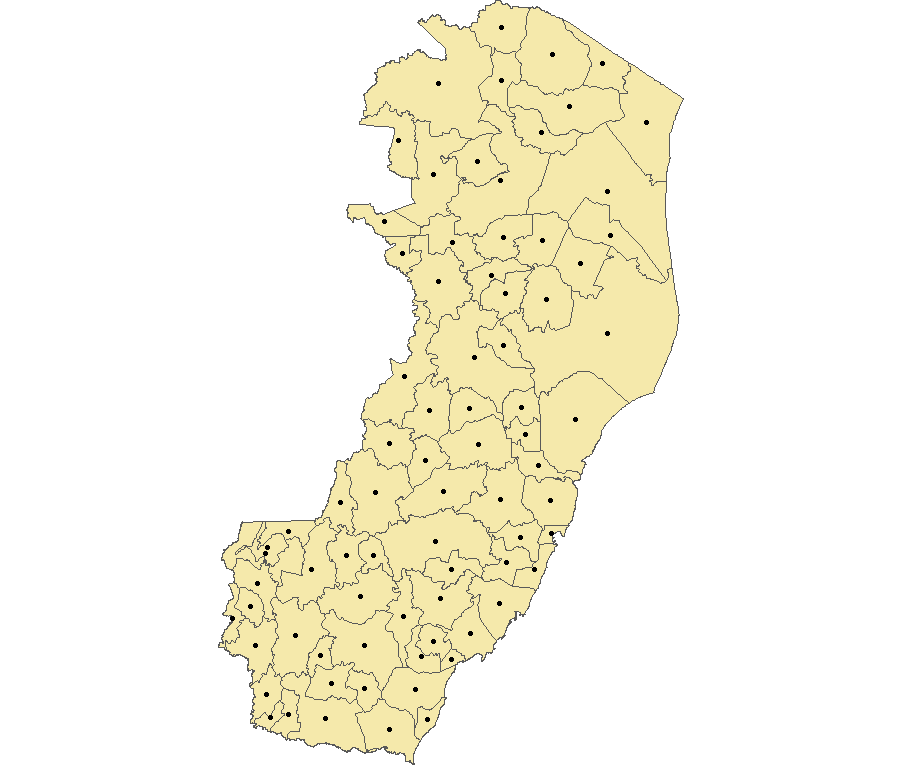
\includegraphics[width=\linewidth]{images/ES_map.png}
  \caption{Mapa apenas com os municípios e seus respectivos centroides.}
  \label{fig:ES}
\end{subfigure}%
\begin{subfigure}{.5\textwidth}
  \centering
  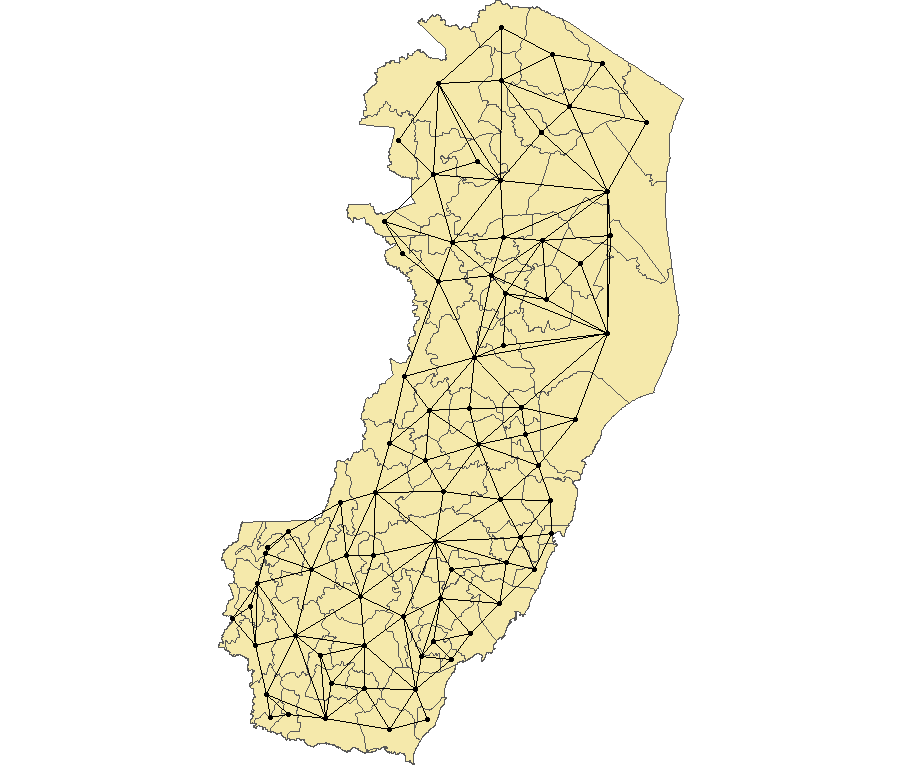
\includegraphics[width=\linewidth]{images/ES_map_conectedgraph.png}
  \caption{Mapa com as relações de vizinhança representadas por um grafo conexo.}
  \label{fig:ES_conexo}
\end{subfigure}
\caption{Mapa dos municípios do Espírito Santo.}
\label{fig:ES_mapas}
\end{figure}

A matriz de adjacências deste grafo é um exemplo de matriz de proximidades.
Uma matriz de proximidades $W$ possui entradas $w_{ij}$ que de alguma forma representam a conexão espacial entre duas regiões $i$ e $j$ (é de costume que $w_{ij} = 0$ se $ i=j$).
Para a matriz de vizinhança, temos $w_{ij} = 1$ se $i\sim j$, e $w_{ij} = 0$ caso contrário.
Há aqui diversas possibilidades para as escolhas de $w_{ij}$, que não necessariamente representam conectividade, como por exemplo $w_{ij}$ ser a distância entre os centroides de $i$ e $j$.
Podemos tomar $w_{ij}  = 1$ se $i$ e $j$ se a distância mínima entre suas fronteias está dentro de um limite pré-estabelecido.
Poderíamos padronizar as linhas de $W$ para torná-la uma matriz estocástica.
O último exemplo acabaria com uma propriedade excelente para uma matriz de proximidades que é ser simétrica. Matrizes de proximidade terão um papel importante para definir a estrutura espacial de nossos modelos.

% Anselin and Griffith (1988) and Arbia  (1989)

E por relacionados para duas entidades geográficas, o que queremos dizer?
No mínimo, esperamos alguma correlação, positiva ou negativa.
Mais do que isso, estarem espacialmente correlacionadas.
Para isso precisamos de técnicas quantitativas para analisar a correlação entre duas variáveis relativa à distância entre as duas ou a conectividade.
Falhar ao levar em conta efeitos espaciais, ou até mesmo ignorá-los pode acarretar em sérios erros na interpretação de modelos como notam \cite{Anselin1988} e \cite{Arbia1989}.
Duas estatísticas padrão para medir a associação espacial entre dados em área são o I de Moran \cite{Moran1950} e o C de Geary \cite{Geary1954}.
São um único valor tentando sumarizar toda associação espacial presente nas áreas.
Para áreas $B = \{1, \dots, n\}$ com observações $Y_i$ para a área $i$, e $w_{ij}$ as entradas da matriz de vizinhança, o I de Moran é dado por

\begin{equation}
    I = \frac{n \sum_{i=1}^n \sum_{j=1}^n w_{ij} (Y_i - \Bar{Y})(Y_j - \Bar{Y})}{(\sum_{i \neq j} w_{ij})\sum_{i=1}^n(Y_i - \Bar{Y})^2},
\end{equation}

e o C de Geary por

\begin{equation}
    C = \frac{(n-1) \sum_{i=1}^n \sum_{j=1}^n w_{ij} (Y_i - Y_j)^2}{2(\sum_{i \neq j} w_{ij})\sum_{i=1}^n(Y_i - \Bar{Y})^2}.
\end{equation}

Estas estatísticas podem ser utilizadas para realizar testes estatísticos.
O I de Moran, sob a hipótese nula que os dados são variáveis i.i.d, é assintoticamente normal com média $-1/(n-1)$.
O C de Geary caso assuma valores baixos entre $(0,1)$ indica a presença de associação espacial.
Assim como o I é assintoticamente normal caso as variáveis sejam i.i.d mas o uso dessas métricas é sugerido apenas como medida exploratória \cite{Li2007}.

Uma forma mais moderna de analisar a dependência espacial de um conjunto de dados é entender que cada unidade de área possui uma quantidade intrínseca de dependência espacial devido à sua situação relativa ao resto do sistema -- ao contrário do I de Moran e do C de Geary, que fornecem uma única medida crua para o sistema inteiro.
A exemplo, temos as estatísticas $G_i$ e $G_i^*$ de \cite{GetisOrd1992}, sobre as quais não entrarei em detalhes.

%Moran's Index	0,145624
%Expected Index	-0,038462
%Variance	0,015644
%z-score	1,471797
%p-value	0,141076

Para exemplificar o uso do I de Moran como ferramenta de detecção de dependência espacial, veja na Figura \ref{fig:pt} o mapa do segundo turno das eleições de 2010 no Brasil.
Calculando o I de Moran para a porcentagem de votos úteis do PT (Partido dos Trabalhadores) e métrica de distância a matriz de vizinhanças, obtemos o valor de $0.1456$ contra o esperado sobre hipótese nula de $-0,0385$, indicando associação espacial entre os estados que elegeram o PT.

\begin{figure}
    \centering
    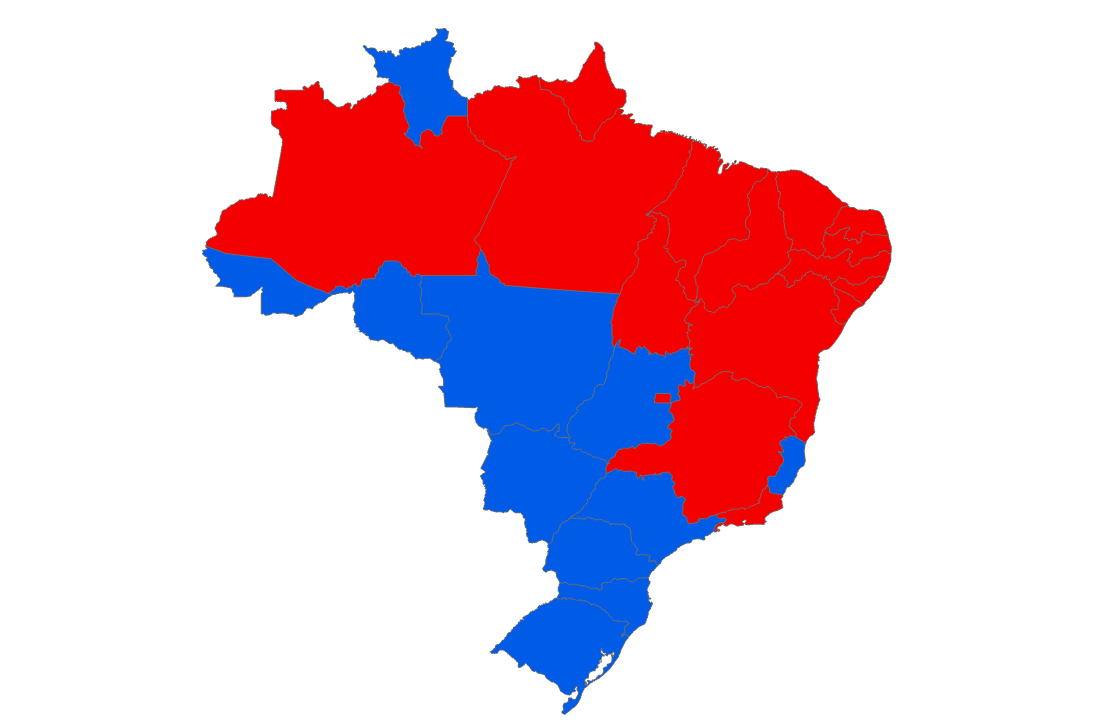
\includegraphics[width = 0.8\linewidth]{images/eleicoes_2010.png}
    \caption{Resultados das eleições de 2010 no Brasil. Em vermelho, estados onde o PT conquistou maioria dos votos. Em azul, maioria do PSDB.}
    \label{fig:pt}
\end{figure}

\cite{Cliff1981} detalha o cálculo de $\mathds{E}[I]$ e $Var(I)$ sob hipótese de normalidade assintótica e de aleatorização.
Aleatorização acontece pois sob hipótese nula não há associação espacial, então permutar as variáveis não modifica a distribuição do $I$ de Moran.
É possível então calcular o \textit{Z-score} e realizar um teste de hipótese.
O teste é implementado em R no pacote \textbf{spdep} como a função \textit{moran.test}.

\subsection{Modelando contagem de casos de uma doença}
% Progressivly explain the Poisson Model?

Para o restante do capítulo, considere a notação $B = \{1, \dots, n\}$ um conjunto de regiões disjuntas, $\delta_i$ o conjunto de vizinhos da região $i$ e $n_{\delta_i}$ o tamanho de $\delta_i$ e $w_{ij}$ como as entradas da matriz de vizinhança $W$.
Dados em área são objetos de forte interesse da Bioestatística e da Epidemiologia.
Tipicamente nos deparamos com dados de contagem de casos por região da seguinte forma:
\[Y_i \quad = \quad \text{casos observados na região $i$,}\quad i=1,\dots,n\]
\[E_i \quad = \quad \text{valor esperado de casos na região $i$,}\quad i=1,\dots,n\]

$Y_i$ variáveis aleatórias e $E_i$ função do número de pessoas em risco na região $i$. 

% Comentar internal standardization

Caso a doença não seja rara \cite{Banerjee2015}, o modelo mais usual é o de Poisson:

\begin{equation}
    \label{eq: poisson}
    Y_i|\theta_i \sim \operatorname{Poisson}(E_i \theta_i),
\end{equation}

onde $\theta_i$ é o risco relativo da região i. Para efeticamente mapear uma superfície de risco, podemos pensar em um modelo de efeito aleatório para os $\theta_i$.
Além de poder assumir que os riscos de cada região vêm de uma mesma distribuição, podemos agregar informação de todas as regiões nas estimativas de risco para uma única região. Também podemos introduzir informação de covariáveis modelando este risco relativo

Considere, então, o seguinte aprimoramento do modelo simples de Poisson, que introduz uma distribuição comum para os $\theta_i$.  

\begin{equation}\label{eq: lognomal}
\begin{split}
    Y_i|\theta_i &\sim \operatorname{Poisson}(E_i \theta_i),\\
    \log(\theta_i) &= \sum_{j=1}^P X_{ij}\beta_j + \varepsilon_i,\\
    \boldsymbol{\varepsilon} &\sim \operatorname{Normal}(0,\Sigma).
\end{split}
\end{equation}

A (log) taxa relativa é modelada como uma componente linear, que introduz informação de covariáveis para o modelo, acrescida de ruído. Aqui $\mathbf{X}$ é uma matriz $N \times P$ com informação de $P$ covariáveis para cada uma das $N$. O ruído modela a sobredispersão, fenômeno muito comum em dados ecológicos e biologia evolucionária \cite{Harrison2014-up}. Esta sobredispersão pode ocorrer devido a covariáveis que não foram incluídas no modelo, excesso de zeros e dados não independentes. Esse rúido é chamado de Efeito Aleatório a Nível Observacional, ou  ORLE (\textit{Observational Level Random Effects}), e ameniza os problemas da sobredispersão descritos. 

% Mix of text from Wakefield and Riebler

Devido à típica incerteza vinda da amostragem, não é recomendado que se analise as taxas diretamente, mas sim tomar ``emprestado'' informação de regiões vizinhas. Espera-se que regiões próximas apresentem mais similaridades que regiões distantes, e é interessante explorar essa informação para extrair estimativas de risco fidedignas.
O efeito é similar a introduzir covariáveis que apresentem tal comportamento: assumem valores similares em locais próximos.
Surge então uma dificuldade para modelar esta dependência espacial, que é conseguir compensar estas covariáveis não observadas e tentar simular seus comportamentos. 

%Riebler
Uma das formas mais comuns de introduzir correlação espacial para um modelo como a Eq. \eqref{eq: lognomal} é com um \textit{Campo de Gaussiano de Markov Intrínseco} (IGMRF), que aqui refiro como modelo CAR (ou termo CAR).
Especificamos a distribuição de um modelo CAR $\boldsymbol{\nu}$ através de suas condicionais completas

\begin{equation*}
    \nu_i | \nu_{-i} \sim \operatorname{Normal}\left(\frac{1}{n_{\delta_i}}\sum_{j \in \delta_i} \nu_j, \frac{1}{n_{\delta_i} \kappa_i}\right),
\end{equation*}

onde $\kappa_i \in (0,+\infty)$ é um parâmetro de precisão.
A partir do Lema de Brook (Lema~\autoref{lema:brook}), e assumindo $\kappa_i = \kappa$ comum parar todas as regiões, podemos derivar a distribuição conjunta de $\nu$:

\begin{equation}
\label{eq: full conditional}
    \pi(\boldsymbol{\nu}|\kappa) \sim \operatorname{Normal}\left(-\frac{1}{2\kappa^2} \sum_{i \sim j} (\nu_i - \nu_j)^2\right) = \operatorname{Normal}\left(\frac{1}{2\kappa^2} \nu^T (D_W - W)\nu \right),
\end{equation}

onde $D_W$ é uma matriz diagonal com entradas $n_{\delta_i}$.
O modelo é intrínseco pois $(D_W - W)1 = 0$, portanto a matriz de precisão é singular e a deficiência de posto é 1 caso o grafo seja conexo, vide \autoref{ap: IGMRF}.
Note também que a densidade é invariante à adição de uma constante, portanto para que não haja confusão com o intercepto, impomos a restrição $\sum_i Y_i = 0$.
Por ser impróprio, vide \autoref{ap: IGMRF}, os modelos CAR intríscos (ICAR) não podem ser usados para modelar dados, e portanto são designadas como prioris.
\cite{Besag1991} mostra que apesar do modelo ser impróprio, a posteriori é própria.

Uma forma de lidar com a condição imprópria do modelo é adicionar um parâmetro $\rho$ escalando a componente $W$  de $(D_W - W)$, controlando então a contribuição espacial deste termo ($W$ é a matriz de vizinhanças). Veja que com $\rho = 0$ temos uma matriz diagonal e, portanto, entradas independentes. Com $\rho = 1$ temos o modelo ICAR. 

\begin{equation}
    \pi(\boldsymbol{\nu}|\kappa) \sim \operatorname{Normal}\left(\frac{1}{2\kappa^2} \nu^T (D_W - \rho W)\nu \right),
\end{equation}

Note que agora tomando $\rho \in (\frac{1}{\lambda_{min}}, \frac{1}{\lambda_{max}})$ obtemos um modelo próprio, onde $\lambda_{min}, \lambda_{max}$ são o menor autovalor e o maior autovalor de $(D_W - \rho W)$, respectivamente
Note que $\rho = 0$ implica em variáveis $\nu_i$ independentes, assim como $\rho = 1$ implica no modelo ICAR.
Apesar de tornar o modelo próprio, permitindo práticas como simulação \textit{a priori} do modelo, o modelo próprio, como alertam \cite{Banerjee2015}, não traz a maleabilidade desejada para introduzir padrões espaciais significativos. 

% Introduzir imagens com simulações de um modelo CAR próprio junto do I e do C


\textcite{Besag1991} introduziram de forma pioneira regressões de Poisson com erros tanto não-estruturados como com erros estruturados de natureza espacial.
O modelo é conhecido como modelo de BYM (Besag-York-Mollié).
Sua formulação é a que segue:

\begin{equation}
    \label{eq: bym}
        Y_i|\theta_i \sim \operatorname{Poisson}(E_i \theta_i),
\end{equation}
\[\log(\theta_i) = \sum_{j=1}^P X_{ij}\beta_j + \xi_i,\]
\[\xi_i = \varepsilon_i + \nu_i,\]
\[\varepsilon_i \sim \operatorname{Normal}(0,\tau_u),\]
\[\nu_i | \nu_{-i} \sim \operatorname{Normal}\left(\frac{1}{n_{\delta_i}}\sum_{j \in \delta_i} \nu_j, \frac{1}{n_{\delta_i} \tau_s}\right).\]

$\tau_s$ e $\tau_u$ parâmetros de precisão.
Note que estes parâmetros de precisão não podem ser vistos de forma independente.
Temos uma observação por área para tentar estimar dois parâmetros! 


\cite{Leroux} e \cite{Dean} trouxeram reparametrizações do modelo BYM para lidar com estes problemas.
Considere a notação $Q = (D_W - W)$ O modelo de Leroux propõe um compromisso entre a componente estruturada e a componente não estruturada por um parâmetro de mistura $\phi \in [0,1]$. O modelo é o BYM mas a componente $\boldsymbol{\xi}$ segue uma distribuição normal com média zero e matriz de covariância

\begin{equation}
\label{eq:leroux}
    \operatorname{Var}(\boldsymbol{\xi}|\tau_b, \phi) = \tau_b^{-1} \left((1-\phi)I + \phi Q  \right)^{-1}.
\end{equation}

A variância condicional do modelo de Leroux é dado pela média ponderada por $\phi$ de $1/\tau_b$ e $1/(\tau_bn_{\delta_i})$.
Como consequência, a decomposição aditiva da variância acontece na log escala do risco relativo condicional à vizinhança da região analisada \cite{Leroux}. O modelo de Dean propõe uma reparametrização do termo $\xi$ do modelo BYM como:
\begin{equation}
\label{eq:dean}
\boldsymbol{\xi} = \frac{1}{\sqrt{\tau_b}}\left( \sqrt{1-\phi}\cdot \boldsymbol{\varepsilon} + \sqrt{\phi} \cdot  \boldsymbol{\nu} \right),
\end{equation}

tendo matriz de covariância
\begin{equation}
    \label{eq:var_dean}
    Var(\boldsymbol{\xi}|\tau_b, \phi) = \tau_b^{-1}\left((1-\phi)I + \phi Q^- \right)
\end{equation}

Onde $Q^-$ denota a inversa generalizada. Esta reparametrização é o modelo BYM com $\tau_s^{-1} = \tau_b^{-1} \phi$ e $\tau_u^{-1} = \tau_b^{-1} (1 - \phi)$. A decomposição aditiva da variância está na log escala do risco relativo.\\

Apesar dos modelos de Leroux e Dean lidarem com a identificação de como a sobredispersão se distribui entre componente estruturada e não estruturada, ambos possuem o problema da componente espacial não estar escalada. Como nota \cite{SORBYE2014}, escalar a componente espacial é essencial para a escolha das prioris, e garantir que as escolhas de priori de uma aplicação possam ser utilizadas em outras aplicações. 

\cite{Ribler2019} detalha o desenvolvimento de um novo modelo BYM, que se atenta à escala. Por simplicidade, considere $\xi$ composto apenas pela componente espacial. Geralmente, as variâncias marginais $\tau_b [Q^-]_{ii}$ dependem da estrutura do grafo analisado. Isso pode ser ilustrado calculando uma variância generalizada, como a média geométrica das variâncias marginais

\begin{equation}\label{eq: GV}
    \sigma^2_{GV} = \exp \left( \frac{1}{n} \sum_{i=1}^n \log \left(  \frac{1}{\tau_b}[Q^-]_{ii}\right) \right).
\end{equation}

Para unificar a interpretação de $\tau_b$ da componente estruturada e da não estruturada, e torná-la transferível entre aplicações, o efeito espacial precisa ser escalado para que $\sigma^2_{GV} = 1/\tau_b$. Isso faz com que o parâmetro $\tau_b$ represente o desvio de um nível constante para qualquer que seja o grafo por trás do modelo. \cite{GMRF} apresenta um esquema para de forma eficiente calcular as entradas da diagonal de $Q^-$. Após extraídos estes componentes, $\sigma^2_{GV}$ é calculado como na \autoref{eq: GV} e é usado para escalar a matriz Q. A partir disso, \cite{Simpson2015}  propõe uma nova parametrização do modelo BYM, que recebe o nome de BYM2. Essa nova parametrização utiliza a componente espacial escalada com precisão 1. O efeito aleatório agora é formulado como

\begin{equation}\label{eq: bym2err}
    \boldsymbol{\xi} = \frac{1}{\sqrt{\tau_b}} \left( \sqrt{1-\phi} \cdot \boldsymbol{\varepsilon} \sqrt{\phi} \cdot \boldsymbol{\nu}^* \right)
\end{equation}

A nova variância é dada por:

\begin{equation}\label{eq: bym2var}
    \operatorname{Var}(\boldsymbol{\xi}|\tau_b, \phi) = \tau_b^{-1}((1-\phi)I + \phi Q_*^-)
\end{equation}

Veja que agora os hiper-parâmetros $\tau_b$ e $\phi$ tem interpretação clara e não são mais confundidos. 

\subsubsection{Escolha das prioris}

Uma questão importante em modelagem bayesiana em geral, e em modelagem espacial em particular é a escolha das distribuições \textit{a priori}.
Modelos GMRF em particular podem ser particularmente sensíveis à especificação de prioris.
%No que se segue, discuto a análise das prioris \textit{via} simulações preditivas.
\textcite{Wakefield2007} trás uma ótima revisão para o caso de regressões espaciais. Par um link log-linear, como é o caso dos modelos estudados nesta seção, é conveniente especificar prioris lognormais para os parâmetros positivos $\exp(\beta_j)$, e fica bem idreto especificar dois quantis e encontrar os parâmetros associados da distribuição lognormal. Denote por $LN(\mu, \sigma)$ a distribuição da lognormal para um parâmetro genérico $\theta$, com $\mathds{E}[\log(\theta)] = \mu$ e $Var(\log(\theta)) = \sigma^2$. Por exemplo, supondo que o risco relativo de uma variável $\beta_j$ tem 50\% de chance de ser menor que 1, podemos assumir \textit{a priori} $\mu = 0$. E uma alta chance, de por exemplo 95\%, de ser menor que 5. Daí $\sigma = \log 5 / 1.645 = 0.98 \approx 1$. Uma priori $e^{\beta_j} \sim LN(0, 1)$ pode ser uma boa escolha. Caso existam muitas covariáveis, ou existe alta correlação entre as covariáveis, vale a pena tornar a priori mais informativa. Como exemplo, veja \cite{IsingDP} que usa prioris de Ising para encorajar a clusterização de variáveis correlacionadas.


Prioris para os parâmetros de precisão do risco relativo residual já não são tão diretas de se derivar. A escolha da distribuição $Gama(a,b)$ para a precisão tanto da componente estruturada, como da não estruturada, ou do risco relativo residual escaldo como no BYM2, é conveniente pois produz uma distribuição marginal em forma fechada. Em especial, sabemos que o modelo de dois níveis
\begin{equation*}
    \xi_i|\tau \sim \operatorname{Normal}(0, 1/\tau), \quad \tau \sim \operatorname{Gama}(a,b)
\end{equation*}

produz distribuição marginal para $\xi_i$ como uma \textit{t}-student generalizada $t_{2a}(0, b/a)$ com $2a$ graus de liberdade, locação zero e escala $b/a$. Uma forma para determinar $a$ e $b$ é especificar um alcance $\exp(\pm R)$ para que o risco residual fique dentro com probabilidade q, e usamos a simetria da t para obter que $\pm t_{q/2}^{2a} \sqrt{b/a} = \pm R$, Onde $\pm t_{q/2}^{2a}$ é o quantil q da t generalizada. Por exemplo, suponha que o risco relativo fique dentro do intervalo (0.5, 2.0) com probabilidade de 95\% , então obtemos que $\tau \sim \operatorname{Gama}(1,0.026)$. 

É importante garantir que a priori acesse todos os possíveis níveis de variabilidade no resíduo. Por esta razão \textcite{Wakefield2007} não recomenda o uso de prioris vagas como $\operatorname{Gama}(0.001,0.001)$.

\subsubsection{Simulações}

Os termos CAR conseguem compensar por covariáveis espacialmente associadas e controlar pela correlação espacial do ruído.
Para ilustrar o fato, considere o seguinte exemplo artificial. Gerei uma covariável $x^*$ com clara dependência espacial para o mapa do Espírito Santo como mostra a \autoref{fig:ES_G}. Em adição foram geradas duas covariáveis $x_1, x_2$ de uma normal padrão para cada região.
A quantidade de interesse $Y$ é então obtida pondo $Y_i \sim \operatorname{Poisson}(\theta_i)$, e $\log(\theta) = 1.5 + 0.5x_1 -0.5x_2 + 0.3x^*$. Vamos amostrar de dois cenários diferentes, desconsiderando a variável $x^*$: o primeiro um modelo Poisson log-normal simples, e o segundo o mesmo modelo com um termo CAR.
Para medir a associação espacial no resíduo utilizo o teste de Moran.
\begin{figure}[ht]
    \centering
    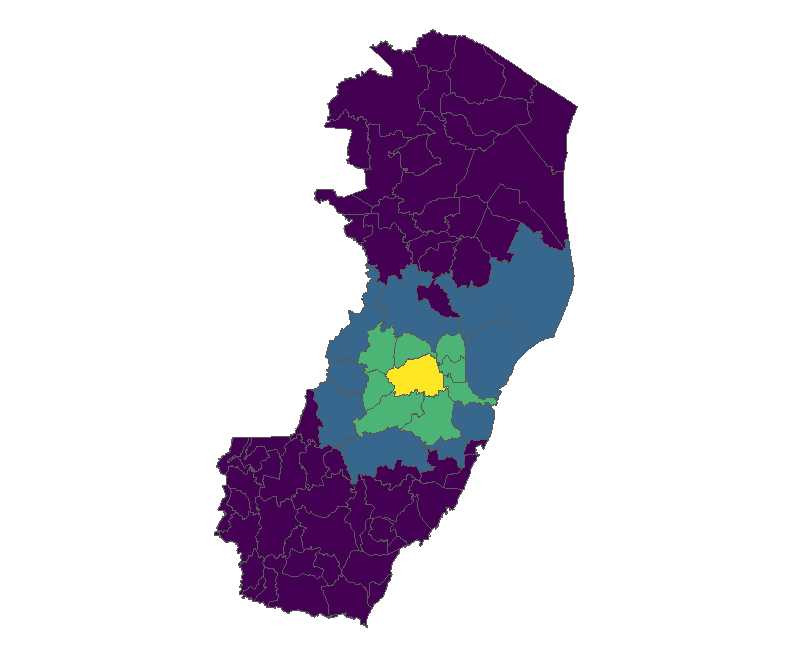
\includegraphics[width = 0.6\linewidth]{images/ES_G.png}
    \caption{Covariável espacialmente correlacionada gerada artificialmente para o mapa do Espírito Santo. }
    \label{fig:ES_G}
\end{figure}
Para o modelo tradicional o I de Moran no resíduo vale 0.194, contra o esperado sobre hipótese nula de -0.013 e um p-valor de 0.0025. Para o modelo com termos CAR o I de Moran no resíduo vale -0.04 contra um esperado de -0.13 e um p-valor de 0.70. 

Um segundo experimento é verificar se as reparametrizações de Dean, Leroux e o BYM2 reduzem aos modelos básicos, i.e, num cenário de alta correlação espacial o parâmetro de mistura $\phi$ se aproximar de 1, no caso de efeitos regionais aleatórios $\phi$ se aproximar de zero. Para isso, simulo do modelo de Poisson com $\log(\theta_i) = 0.4 + 0.5 \xi_i$. Suponho três cenários: $\xi_i$ vindo de uma normal padrão, $\xi$ tendo distribuição $N(0,Q_*^-)$, onde $Q_*$ é a matriz $Q$ escalada para o grafo de adjacências do Espírito Santo, e um terceiro que é uma superfície de risco constante. O modelo avaliado é o BYM2. A priori para o parâmetro $\phi$ é a da indiferença $U(0,1)$.
Os resultados estão apresentados na \autoref{tab:posterior_summary_sim}. Veja que para o modelo de superfície constante o BYM2 a posteriori de $\rho$ não se distancia muito da priori. Já para os cenários de 2 e 3 o parâmetro $\rho$ já apresenta um desvio da priori imposta. Não houve uma redução completa para $\phi = 0$ ou $\phi = 1$. \cite{Simpson2015} propõe o uso de prioris penalizadoras de complexidade (prioris PC) para o BYM2 que conseguem reduzir o parâmetro de mistura para zero. Prioris PC são baseadas na Navalha de Ockham - modelos mais simples devem ser preferidos até que se tenha evidência o suficiente para um modelo mais complexo. 


\begin{table}

\centering
\begin{tabular}{@{}lrrcrrccc@{}}\toprule
& \multicolumn{2}{c}{$\beta_0$} & \phantom{ab}& \multicolumn{2}{c}{$\rho$}&\phantom{ab}& \multicolumn{2}{c}{$\frac{1}{\sqrt{\tau}}$}\\

%\cmidrule{2-3} \cmidrule{5-6}
%& $Média$ & $(upp,lwr)$ && $Média$ & $(upp,lwr)$\\
\midrule
\textbf{Cenário 1} & 0.32 & (0.10) && 0.51 & (0.29) && 0.28 &(0.10)\\
\textbf{Cenário 2} & 0.45 & (0.10) && 0.36 & (0.29) && 0.40 &(0.16)\\ 
\textbf{Cenário 3} & 0.43 & (0.10) && 0.68 & (0.14) && 0.54 &(0.14)\\ 
\bottomrule
\end{tabular}
    \caption{Sumários à posteriori para os 3 cenários descritos: superfície de risco constante, superfície de risco com efeito aleatório regional e superfície de risco com efeito aleatório espacial. Para cada parâmetro temos a mediana à posteriori junto com o desvio-padrão.}
    \label{tab:posterior_summary_sim}
\end{table}





\section{Seleção de Variáveis}

Ao lidar com um conjunto de preditores num termo linear, junto com a estimação dos coeficientes é comum também determinar quais destes preditores estão mais associados com a variável a ser predita. Para o caso de $P$ preditores, queremos determinar um ``bom'' submodelo dentre os $2^P$ submodelos possíveis, baseado em algum critério apropriado .  Para modelos Bayesianos, uma métrica comum para a comparação de modelos é o WAIC (Widely Applicable Information Criterion) \textcite{WAIC}. Usando a mesma notação da \autoref{sec:spatial} para modelos de contagem de casos, considere uma variável de exposição $Y$ para $N$ regiões e um conjunto de $P$ preditores $X = (X_1, \dots, X_p)$ e $\theta$ todos os parâmetros de interesse.
O WAIC  do modelo é calculado como
\begin{equation}
\label{WAIC}
    \operatorname{WAIC} = \mathds{E}[D(\theta)] + 2\sum_{i=1}^N \log(\mathds{E}[p(Y_i|\theta)]) - \mathds{E}[\log p(Y_i|\theta)],
\end{equation}
\[\mathds{E}[D(\theta)] = -2\log(p(Y|\theta))\].

Tem a vantagem de poder ser calculado sem assumir nenhuma distribuição ``verdadeira'', e funciona como um \textit{cross-validation} Bayesiano medindo o poder preditivo do modelo fora da amostra. No entanto, para o trabalho de seleção de variáveis, onde o espaço de modelos cresce exponencialmente com o número de covariáveis, é inviável executar essa computação para todos os modelos.

Do ponto de vista Bayesiano, este problema é contornado ao considerar a seleção de variáveis como uma forma de estimação de parâmetros. A ideia básica é definir as variáveis latentes $\boldsymbol{\gamma} = \{\gamma_i, 1 \leq i \leq P\}$ onde $\gamma_i$ é uma variável indicadora da inclusão do i-ésimo preditor $X_i$ no modelo. Em muitos casos, a decisão de incluir ou não uma variável recai na estimação da probabilidade marginal à posteriori de incluir uma variável no modelo (probabilidade marginal à posteriori dos parâmetros $\gamma_i$). \cite{Ohara2009} traz uma revisão de diversas formas de incluir esta seleção de variáveis para o problema de regressão Bayesiana. Mantendo a notação da \autoref{sec:spatial}, considere agora a seguinte versão aumentada do termo linear da \autoref{eq: lognomal}

\begin{equation}
\begin{split}
        \log(\theta_i) &= \beta_0 + \sum_{j=1}^{P} X_{ij} \nu_j + \varepsilon_i,\\
        \nu_j|\gamma_j, \beta_j &\sim G.
\end{split}
\end{equation}

A tarefa de seleção de variáveis então se simplifica a decidir quais dos parâmetros $\nu_j$ valem zero. A distribuição condicional $G$ seguem, então, a forma de uma mistura ``spike-and-slab'' (pico e platô), possuindo um pico de densidade em zero e um platô de densidade nos outros pontos. Aqui considero dois casos para a densidade $G$. A primeira, de \cite{KM1998} e que me refiro por seleção de variáveis por indicadoras, de forma simples e direta atribui $\nu_j = \gamma_j \beta_j$, e prioris independentes para $\boldsymbol{\gamma}$ e $\boldsymbol{\beta}$. A segunda, inicialmente proposta por \cite{McCulloch1993} e que me refiro como SSVS (Stochastic Search Variable Selection), atribui $\nu_j = \beta_j$ e altera a distribuição de $\beta_j$ baseado nas indicadoras da seguinte forma

\begin{equation}
    \beta_j|\gamma_j \sim (1- \gamma_j) N(0,\sigma^2) + \gamma_j N(0, c_j^2\sigma^2).
\end{equation}


Aqui o pico é uma distribuição centrada em zero com baixa variância, e o parâmetro de $\sigma^2$ é calibrado para que isso aconteça. $c_j$ é calibrado para garantir o platô da distribuição. 

Para todos os casos a escolha da priori para $\gamma$ é parte essencial do problema. Essa escolha deve incorporar qualquer informação prévia sobre os modelos mais plausíveis. No entanto, com $2^P$ modelos isto se torna uma tarefa complexa. Para $\gamma_i$'s independentes com distribuição marginal Bernoulli com $P(\gamma_i = 1) = p_i$ a densidade conjunta de $\gamma$ vale:

\begin{equation}\label{eq:joint_density_gamma}
f(\boldsymbol{\gamma}) = \prod_{i = 1}^{P} p_i^{\gamma_i}(1-p_i)^{1-\gamma_i}.
\end{equation}

Algumas hipóteses de simetria podem facilitar nossa atribuição da priori. A priori uniforme, ou priori da indiferença, é dada por:

\begin{equation}
    f(\boldsymbol{\gamma}) = 2^{-p}.
\end{equation}

Com $p_i = \frac{1}{2}$ para todo $i \in \{1,\dots,P\}$. Podemos também penalizar o tamanho do modelo $M_{\gamma} = \sum_{i=1}^{p} \gamma_i$  pondo mais densidade a priori em modelos menores, favorecendo a parcimônia. Umas das sugestões de \cite{McCulloch1993} é colocar

\begin{equation}
    f(\boldsymbol{\gamma}) = w_{M_{\gamma}} \binom{P}{M_{\gamma}}^{-1},
\end{equation}

onde $w_{M_{\gamma}}$ é a probabilidade a priori de obter um modelo de tamanho $M_{\gamma}$. Para controlar o tamanho do modelo, \cite{Carvalho2019} sugere a parametrização de $p_i$ pela maleabilidade do modelo. Um modelo nada maleável não inclui nenhuma covariável. Seja $w = P(M_{\gamma} = 0)$ nosso parâmetro de maleabilidade. Considerando que $p_i = q, i \in \{1,\dots, P\}$, é fácil ver que $w = (1-q)^P$, e então $q = 1 - w^{1/P}$.

Uma vantagem desta formulação é poder rapidamente avaliar a importância de uma variável por meio do Fator de Bayes de $\gamma$. Podemos escrever o Fator de Bayes para a i-ésima covariável como a razão da razão de chances à posteriori com as chances à priori:

\begin{equation}\label{eq: BF}
BF_i = \frac{\hat{\gamma_i}}{1 - \hat{\gamma_i}}/\frac{p_i}{1-p_i},
\end{equation}

onde $\hat{\gamma_i)}$ é um estimador da probabilidade à posteriori $\gamma_i$.
Para o caso da SSVS, precisamos também definir prioris para $\sigma$. $\sigma$ deve ser tal que $\beta_j \sim N(0,\sigma^2)$ pode ser seguramente substituído por zero. Note que o parâmetro $c_i$ representa a razão das alturas de $N(0,\sigma^2)$ e $N(0,c_i^2\sigma^2)$ em 0. Portanto, pode ser interpretado como a razão de chances de $\beta_i$ ser excluído quando assume valores próximos de 0.  \cite{McCulloch1993} propõe uma alternativa semi-automática, utilizando informação do estimador de mínimos quadrados para $\sigma$. Prefiro não utilizar tal abordagem, adotando prioris mais generalistas para não comprometer a característica Bayesiana completa dos modelos. 

Por fim, precisamos detalhar a escolha de priori para $\beta|\gamma$. Priori para o termo ORLE segue as mesmas recomendações da \autoref{sec:spatial}. Para isso, uso uma normal multivariada

\begin{equation}\label{eq:beta_prior}
    \boldsymbol{\beta}|\boldsymbol{\gamma} \sim N_p(0, D_{\gamma}RD_{\gamma}),
\end{equation}

onde R é a matriz de correlação a priori e 

\begin{equation}\label{eq: Dg}
    D_{\gamma} = \operatorname{diag}[(1-\gamma_1)\tau_1 + \gamma_1 c_1 \tau_1, \dots, (1-\gamma_p)\tau_p + \gamma_p c_p \tau_p].
\end{equation}

Para a escolha de R é interessante observar o efeito dela na matriz de covariância à posteriori de $\beta$, a saber

\begin{equation}\label{eq: posterior_R}
    (\sigma^{-2}X^T X + D_{\gamma}^{-1} R^{-1} D_{\gamma}^{-1})^{-1}.
\end{equation}

Casos notáveis são $R=I$ e $R = (X^T X)^{-1}$. Para o primeiro, os betas ão independentes à priori e as correlações à posteriori serão menores que as correlações da matriz de design. Para o último, correlações à priori e à posteriori serão as mesmas da matriz de design. \cite{McCulloch1993} observa considerável diferença entre ambas as escolhas. Para a escolha $R=I$, modelos menores foram escolhidos com uma maior frequência. 

\subsection{Simulações}

Para avaliar as técnicas de seleção de variáveis vou conduzir algumas simulações artificiais aos moldes de \textcite{VANERP201931}, testando ambos os modelos de Kao e Mallick e o de McCulloch, que me refiro como modelos KM e MC, respectivamente. As simulações são feitas do modelo $y = X^T \boldsymbol{\beta} + \boldsymbol{\varepsilon}, \quad \varepsilon \sim N(0,\sigma^2 I)$ em R com o pacote NIMBLE. Para garantir convergência foi analisado o $\hat{R}$ de Gelman-Rubin, avaliando se o valor para cada parâmetro é menor que 1.05 na última amostra. Todas as cadeias foram executadas com 10.000 iterações, sendo 2.00 usadas como \textit{burn-in}. Como priori para $\sigma^2$ é usado para ambos os modelos uma gama inversa de parâmetros (5,5). Os parâmtros $c$ e $\sigma$ para o modelo MC são fixados como $c = 500$ e $\sigma = 0.01$. Considero que o modelo incluiu uma variável se sua média à posteriori é maior que 0.5


\begin{itemize}
    \item Cenário 1 - $\beta = (3,0,0,-1,0,2,0)$, $\sigma^2 = 9$, X vindo de uma normal multivariada com vetor de média zero, variâncias 1 e correlação entre as variáveis igual a 0.5. São observadas 200 amostras.
    \item Cenário 2 - $\beta = (0.85,0.85,0.85,0.85,0.85,0.85,0.85)$. As outras configurações iguais ao cenário 1.
    \item Cenário 3 - $\beta = (\underbrace{3,\dots,3}_{15},\underbrace{0,\dots,0}_{15})$. $\sigma^2 = 225$. $x_j = Z_1 + w_j,\quad j=1,\dots,5$, $x_j = Z_2 + w_j,\quad j=6,\dots,10$, $x_j = Z_3 + w_j,\quad j=11,\dots,15$, $x_j \sim N(0,1), \quad j=16, \dots 30$. $Z_1, Z_2, Z_3 \sim N(0,1)$ e $w_j \sim N(0,0.01)$. São observadas 200 amostras. 
    \item Cenário 4 - Cenário 3 com 400 amostras.
    \item Cenário 5 - Cenário 3 com $\beta = (\underbrace{3,\dots,3}_{10}, \underbrace{0,\dots,0}_{10}, \underbrace{3,\dots,3}_{10})$ e 40 observações.
\end{itemize}

Para o cenário 1 ambos os modelos geram bons estimadores para os parâmetros da regressão. Já se nota algumas diferenças. O modelo KM ainda tem os betas definidos como zero sendo escolhidos, enquanto o modelo MC rapidamente entende que esses betas não devem ser selecionados. Algo que era esperado, o ESS do modelo MC é menor do que o modelo KM. Para o cenário 2, o modelo KM manteve o mesmo comportamento, aceitando todas as variáveis e fornecendo estimadores razoáveis. Já o modelo MC performou pior, e foi necessário recalibrar os parâmetros $\tau$ e $c$ para obter resultados melhores. Para o cenário 3, o modelo KM incluiu de forma errada 2 variáveis, enquanto do modelo MC incluiu 4 variáveis de forma errada. Para o cenário 4, tivemos4 falsas inclusões para o modelo KM e 6 falsas inclusões para o modelo de MC. Para o cenário 5, 15 falsas inclusões para o modelo de MC e 11 falsas inclusões para o modelo de KM. 

Os resultados das simulações indicam que o modelo de MC precisa de um trabalho mais cuidadoso para a escolha do hiper-parâmetros do problema. Por este motivo, para as simulações praticas utilizo o modelo de KM como método de SSVS. 




\begin{figure}
    \centering
    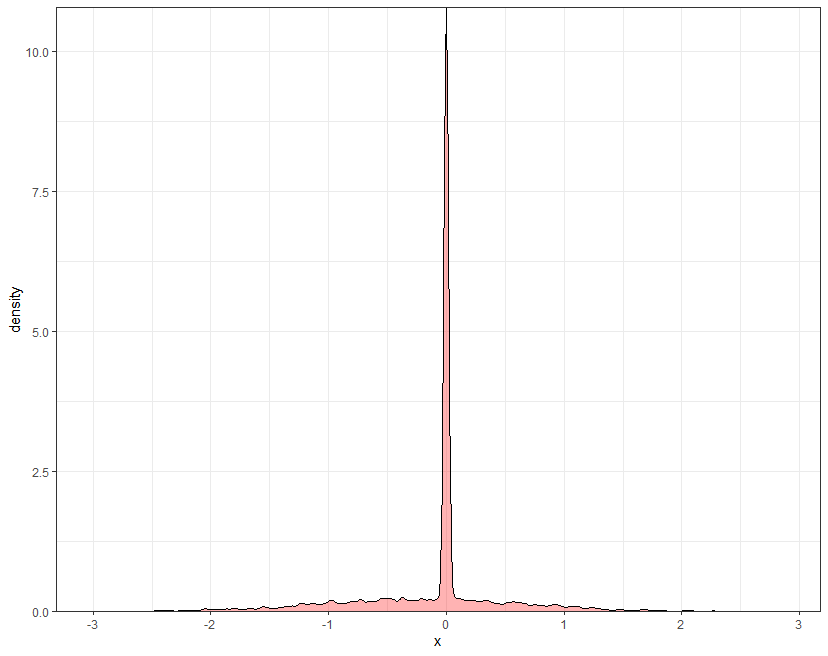
\includegraphics[width = 0.8\linewidth]{images/spike_n_slab2.png}
    \caption{Ilustração da densidade \textit{à posteriori} de uma excluída pra o cenário de simulação 3 para o modelo de Kuo e Mallick. Veja como a concentração de densidade fica em zero, mas o modelo permitiu que ela explorasse outros possíveis valores}
    \label{fig:my_label}
\end{figure}


